\chapter{Introduction to Funnels}
\label{sec:first-app}

This appendix presents funnels from the ground up starting with the Lyapunov
formulations for stability, progressing on to linear stability and finally
introduces \ac{SOS} programming for verifying invariant sets around a fixed
point. All the following sections are based on the lecture notes from
\cite{tedrakeUnderactuatedRoboticsAlgorithms2019}, and are adapted slightly for
presentation in this thesis.

\section{Fundamental Theory}

\subsection{Lyapunov Functions}

A \textit{Lyapunov function} for an autonomous dynamical system is defined as a
scalar function \(V: \R^n \rightarrow \R\), with continuous first derivatives,
which is locally positive definite, and where \(\Delta V \cdot g\) is also
locally negative definite. The \textit{Lyapunov functions} can then be used to
prove the \textit{Lyapunov stability} of the dynamical system. If
\(\dot{\vect{x}} = f(\vect{x})\) is a dynamical system, and \(\dot{V}\) is the
time derivate of the \textit{Lyapunov-candidate function} \(V\), then:
\[
  \dot{V}(\vect{x}) = \frac{d}{dt}V(\vect{x}(t)) = \frac{\partial V}{\partial
    \vect{x}} \cdot \frac{\mathrm{d}\vect{x}}{\mathrm{d}t} = \Delta V \cdot
  \dot{\vect{x}} = \Delta V \cdot f(\vect{x})
\]

\subsection{Lyapunov Stability}

A function being stable in the sense of \textit{Lyapunov}, is defined as: Given
the autonomous nonlinear dynamical system
\[
  \dot{\vect{x}} = f(\vect{x}(t)), \, \vect{x}(0) = \vect{x}_0
\]
where \(\x(t)\) denotes the state vector of the system, with \(\vect{x}(t) \in
\mathcal{D} \subseteq \R^n\). \(\mathcal{D}\) is an open set containing the
origin, and \(f \colon \mathcal{D} \rightarrow \R^n\) continuous on
\(\mathcal{D}\). Suppose that \(f\) has an equilibrium at \(\vect{x}_e\) so that
\(f(\vect{x}_e) = 0\), then this equilibrium is \textit{Lyapunov stable} if for
every \(\epsilon > 0\) there exists a \(\delta > 0\) such that if \(\left \lVert
  \vect{x}(0) - \vect{x}_e \right \rVert < \delta\) then for every \(t \geq 0\)
we have \( \lVert \vect{x}(t) - \vect{x}_e \rVert \leq \epsilon\). Conceptually
this means that a solution starting out in the vicinity of the equilibrium
\(\delta\), will remain close \(\epsilon\) to it. Also note that this must be
true for any \(\epsilon\) one may choose.

\subsection{Lyapunov's Second Method for Stability}

\textit{Lyapunov's} second method (also referred to as \textit{Lyapunov's}
direct method) for stability makes use of the \textit{Lyapunov} function \(V\).
If given a dynamical system of the form \(\dot{\vect{x}} = f(\vect{x})\) having
a point of equilibrium at \(\vect{x} = 0\). Consider a function \(V(\vect{x})
\colon \R^n \rightarrow \R\), such that
\begin{align*}
  V(\vect{x}) &= 0 \text{ if and only if } \vect{x} = 0 \\
  V(\vect{x}) &> 0 \text{ if and only if } \vect{x} \neq 0 \\
  \dot{V}(\vect{x}) &= \frac{d}{dt}V(\vect{x}) = \sum_{i=0}^{n} \frac{\partial V}{\partial \vect{x}_i} f_i(\vect{x}) \leq 0 \text{ for all values of } \vect{x} \neq 0. \\
\end{align*}
Then \(V(\vect{x})\) is called a \textit{Lyapunov function} candidate and the
system is stable in the sense of Lyapunov.

\subsection{LaSalle's Invariance Principle}
\label{subsec:LaSalle's invariance principle}

\textit{LaSalle}'s invariance principle formalizes the convergence of a
dynamical system to an invariant set, rather than to a fixed point. Defined as:
Given a system \(\dot{\vect{x}} = f(\vect{x})\) with \(f\) continuous. If we
produce a scalar function \(V(\vect{x})\) with continuous derivatives for which
over an open subset \(\mathcal{B} \in \R^n\) we have
\begin{align*}
  V(\vect{x}) \geq 0, \; \dot{V}(\vect{x}) \leq 0,
\end{align*}
and \(V(\vect{x}) \rightarrow \infty\) as \(\norm{\vect{x}} \rightarrow
\infty\), then \(\vect{x}\) will converge to the largest \textit{invariant set}
where \(\dot{V}(\vect{x}) = 0\). Where an \textit{invariant set},
\(\mathcal{G}\), of the dynamical system is a set for which \(\vect{x}(0) \in
\mathcal{G} \implies \forall t > 0,\, \vect{x}(t) \in \mathcal{G}\). Meaning
that once you enter the region of invariance, you never leave; which will be
important for calculating funnels.

\subsection{Lyapunov Analysis with Convex Optimization}
\label{subsec:Lyapunov analysis with convex optimization}

One of the primary limitations in Lyapunov analysis is that it is potentially
very difficult to come up with suitable \textit{Lyapunov} function candidates
for under-actuated systems. Even if given a \textit{Lyapunov} function, simply
checking that the \textit{Lyapunov} conditions hold for all \(x\) can be
difficult. Imagine checking that \(\dot{V}\) is strictly negative for all \(x\),
except at the origin, if \(\dot{V}\) is some complicated nonlinear function over
a vector \(x\). A natural approach to a numerical algorithm for verifying
\textit{Lyapunov} stability could be to evaluate \(V\) and \(\dot{V}\) at a
large number of points and check that \(V\) is positive, and that \(\dot{V}\) is
negative. However, this search is slow, and the search space has holes from the
discretization. However with the advances in convex optimization from
\cite{parilloStructuredSemidefinitePrograms}, the possibility to search for a
Lyapunov function numerically now exists. Using optimization algorithms which
rigorously checks these conditions \textit{for all \(x\)}, without the need for
dense sampling. This enables searching for \textit{Lyapunov functions} in an
infinite function space.

\subsection{Lyapunov Analysis for Linear Systems}
\label{subsec:Lyapunov analysis for linear systems}

\begin{theorem}
  Given a linear system of the form \(\dot{\vect{x}} = A\vect{x}\) if one can
  find a \textit{Lyapunov function}
  \[
    V(\vect{x}) = \vect{x}^{T}P\vect{x}, \; P = P^{T} \succeq 0
  \]
  where \(\succeq\) means that the matrix is \ac{PSD}. This also satisfies
  \[
    \dot{V} = \vect{x}^{T}PA\vect{x} + \vect{x}^{T}A^{T}P\vect{x} \succeq 0.
  \]
  Then the origin is globally asymptotically stable.
\end{theorem}

For the linear case the existence of a quadratic \textit{Lyapunov} function is a
neccesary and sufficient condition for stability. Furthermore, a
\textit{Lyapunov} function can always be found by finding the positive definite
solution to the matrix Lyapunov equation
\begin{equation}
  \label{eqn:linearlyapunov}
  PA + A^{T}P = -Q
\end{equation}
for any \(Q = Q^{T} \geqslant 0\).

\subsection{Lyapunov Analysis and Convex Optimization}

The first connection between Lyapunov analysis and convex optimization can be
found through \ac{SDP}-programming. In fact, the Lyapunov conditions for a
linear system can be formulated in the form of a \ac{SDP} problem - which is a
form of convex optimization. For any problem formulated as an \ac{SDP} there
exists an efficient -- and optimal -- solution, barring numerical difficulties.

\subsubsection{Semidefinite Programming}

\begin{figure}
  \centering
  \includegraphics[scale=.5]{figures/preliminaries/Convex_cone_illust}
  \caption[A convex cone illustrated]{A convex cone (light blue). Inside of it, the light red convex cone
    consists of all points \(\alpha x + \beta y \) with \(\alpha,\, \beta > 0\),
    for the depicted \(x\) and \(y\). The curves on the upper right symbolize
    that the regions are infinite in extent.
    \cite{alexandrovConvexConeIllust2019}}
\end{figure}


A wide variety of nonlinear convex optimization problems can be formulated and
efficiently solved as \ac{SDP}s. In control theory, semidefinite programming is
a method for numerically finding the optimal solution of a linear matrix
inequality. It is concerned with the optimization of a linear objective function
over the intersection of the \textit{cone} of positive semidefinite matrices
with an affine space. A convex cone is a subset of a vector space over an
ordered field that is closed under linear combinations with positive
coefficients. A semidefinite program can solve all problems of the form:

\begin{align*}
  \text{minimize } &\textsf{Tr}\,CX \\
  \text{subject to } &\textsf{Tr}\,A_{i}X = b_{i} \text{for all i } = 1,\ldots,m\\
                   &X \succeq 0
\end{align*} 
where \(X \in S^n\), with \(S^n\) being the space of real symmetric \(n \times
n\) matrices. The vector \(\vect{b} \in \R^m\), and the matrices \(A_i \in
S^n\), and \(C \in S^n\) are given problem
parameters~\cite{wolkowiczHandbookSemidefiniteProgramming2000}.

\paragraph{A simple example}
\label{subsec:A simple example}

\begin{figure}
  \centering
  % 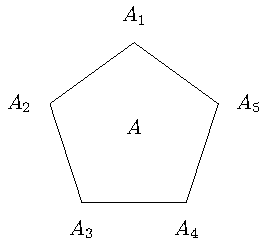
\includegraphics{figures/funnel/linearuncertainlyapunov}
  \documentclass[tikz]{standalone}
\usetikzlibrary{shapes.geometric}

\begin{document}
    \begin{tikzpicture}
      \foreach \a in {5}{
        \node[regular polygon, regular polygon sides=\a, minimum size=3cm, draw] at (\a*4,0) (A) {};
        \node[circle, label=above:\(A_1\)] at (A.corner 1) {};
        \node[circle, label=left:\(A_2\)] at (A.corner 2) {};
        \node[circle, label=below:\(A_3\)] at (A.corner 3) {};
        \node[circle, label=below:\(A_4\)] at (A.corner 4) {};
        \node[circle, label=right:\(A_5\)] at (A.corner 5) {};
        \node[circle, label=\(A\)] at (20,-.35) {};
      }
    \end{tikzpicture}
\end{document}
  \caption[An illustration of the linear search space]{Illustration of the search space.}
\end{figure}

\begin{align*}
  \min{a}\, \text{subject to}
  \begin{bmatrix}
    a & 0 \\
    0 & 1 \\
  \end{bmatrix}
  \succeq 0
\end{align*}
which clearly is \(0\).

Now the linear Lyapunov example from \cref{subsec:Lyapunov analysis for linear
  systems}, can be formulated like a \ac{SDP}:
\begin{align*}
  \text{find P, subject to } P \succeq 0, \; PA + A^{T}P \preceq 0.
\end{align*}
This formulation provides the ground for an automatic search for a
\ac{LQR}-controller. Shown below, is also how one can make it robust to bounded
uncertainties.

This problem formulation can also handle uncertainty, as given the system
\(\dot{\vect{x}} = A\vect{x}\), where \(A\) is unknown, with bounded uncertain
parameters. This set can be described by writing \(A\) as an uncertain linear
combination of known matrices, e.g:
\[
  A = \sum_{i} \beta_{i}A_{i}, \; \sum_{i}\beta_{i} = 1, \; \forall i,\beta_{i}
  > 0
\]
The formulation describes a polygon in the \(A\) space, with each vertex being
one of the \(A_{i}\) which is used to describe \(A\) as a linear combination.

This problem, once formulated can then be sent to an automatic \ac{SDP}-solver,
such as \textit{MOSEK}\cite{mosek}, which is used in this thesis. This example
is important as it provides a way in which to search an infinite function space
numerically. Furthermore, the solution is optimal as long as the problem is
convex. Downside, however, is that this method only works on linear systems, and
the problem at hand in this thesis is nonlinear.

\section{SOS}

In order to extend the functionality to nonlinear systems, the algebraic
geometry theory of \ac{SOS} is necessary. \ac{SOS} is about representing
\textit{non-negative polynomials} as a sum of squares of polynomials. In short,
if one can write a polynomial \(p\) with indeterminates \(x_1,x_2,\ldots,x_n\),
then \(p\) is \ac{SOS} if
\[
  p(\vect{x}) = \sum_{i=1}^{m}g_i^2(\vect{x})
\]
for \(g_i \in \P\), where \(\P\) is the space of polynomials. The clue is that
every form that is \ac{SOS} is also a positive polynomial, although the converse
is not necessarily true~\cite{majumdarFunnelLibrariesRealtime2017}. This is an
important detail, as the numerical search for Lyapunov functions can only verify
\ac{SOS}-polynomials, and as such there will be a \textit{gap} in the Lyapunov
functions we can find and verify, versus the \textit{best} Lyapunov function for
the problem at hand, as there is no guarantee that a \ac{SOS}-Lyapunov function
will be the optimal candidate~\cite{parilloStructuredSemidefinitePrograms}.

\subsection{SOS Programming}

The procedure used to search the space of all positive Lyapunov functions which
can be written as a sum of squares is called \ac{SOS} programming.
With~\citeauthor{parilloStructuredSemidefinitePrograms}'s
work~\cite{parilloStructuredSemidefinitePrograms}, there now exists an efficient
way of restructuring a \ac{SOS} program into an \ac{SDP} program, solve it, then
convert it back, and get the sought solution. \ac{SOS} programming relies on the
ability to write a SOS polynomial in the form
\begin{align*}
  p(\vect{x}) &= s{(\vect{x})}^{T}Qs(\vect{x})\\
\end{align*}
where \(p(\vect{x})\) is a \ac{SOS} polynomial, and \(Q\) is \ac{PSD}, and
\(s(\vect{x})\) is a vector of \textit{monomials} -- meaning that its elements
are the terms in a polynomial, like so
\[
  s(\vect{x}) = \begin{bmatrix} 1 \\ x \\ y \\ x^2 \\ xy \\ y^2 \end{bmatrix}
\]
where \(s(\vect{x})\) is a monomial in \(x\) and \(y\) of order two. In general
\(s(\vect{x})\) is a monomial with degree less than or equal to half that of
\(p(\vect{x})\)~\cite{parilloStructuredSemidefinitePrograms}\label{monomialdegree}.
The condition that \(s(\vect{x})\) is \ac{SOS} is much more
\textit{computationally tractable} than a non-negativity
constraint~\cite{parilloStructuredSemidefinitePrograms}. In this type of problem
the interest lies in finding polynomials \(p_i(\vect{x}), \,
i=1,2,\ldots,\hat{N}\), and sums of squares \(p_i(\vect{x}), \,
i=(\hat{N}+1),\ldots,N\), such that
\[
  a_{0,j}(\vect{x}) + \sum_{i=1}^{N}p_{i}(\vect{x})a_{i,j}(\vect{x}) = 0, \;
  \text{for } j = 1,2,\ldots,J.
\]
where \(a_{i,j}(\vect{x})\) are given constant coefficient polynomials. Problems
of this type is what will be referred to as \ac{SOS} programs throughout this
thesis. The great benefit of \ac{SOS} programming is that it enables the
solution of problems which can be formulated having positivity constraints of
the kind \(f(\vect{x}) \geq 0\).

\subsubsection{A Simple \ac{SOS} Polynomial}
\[
  p = 2 - 8x + 17x^2
\]
which is a sum of squares polynomial, as it can be written in the form
\[
  p = \sum_{i=1}^{N}g_i^2(x) = g_1^2(x) + g_2^2(x) + g_3^2(x)= 1 + {(1-4x)}^2 +
  x^2
\]
which shows that \(p(x)\) is positive for all x. In fact, \(p\) is \ac{SOS} if
and only if there exists a \acl{PSD} matrix \(Q\), such that \(p(\vect{x}) =
s{(\vect{x})}^{T}Qs(\vect{x})\). Which \(p\) is since,
\[
  Q =
  \begin{bmatrix}
    2 & -4 \\
    -4 & 17
  \end{bmatrix}
\]
is a \acl{PSD} matrix.

\subsection{Lyapunov Analysis Using SOS Programming}

With the link shown between positive polynomials and \ac{SOS} programming, it is
time to start looking at the link between Lyapunov functions and SOS
programming. Thus, given a dynamical system of the form \(\dot{\vect{x}} =
f(\vect{x})\), and a Lyapunov function of the form
\[
  V(\vect{x}) = \sum_{i=0}^{d} a_{i}x_{i}
\]
with \(d\) being the degree of the polynomial, a \ac{SOS} program can be
formulated as:
\begin{align*}
  \text{find \(\alpha\)}&, \text{ subject to } V(\vect{x}) \text{ is SOS}\\
  -\dot{V}(\vect{x}) &= -\frac{\partial V}{\partial x}f(\vect{x}) \text{ is SOS}.\\
\end{align*}
and because this is a convex optimization problem, the solver will return a
solution if one exists.

\subsubsection{Example -- The Damped Simple Pendulum}

As a simple example where a search for a polynomial Lyapunov function can be
performed is the \textit{simple pendulum} example. The dynamics of the pendulum
can be described as
\[
  ml^2\ddot{\theta} + mgl \sin{(\theta)} = -b\dot{\theta}
\]
which in vector form can be written as
\begin{align*}
  \dot{\theta}_1 &= \theta_2 \\
  \dot{\theta}_2 &= f(\theta_1,\theta_2) = -\frac{g}{l}\sin{(\theta_1)} -\frac{b}{ml^2}\theta_2
\end{align*}
with \(\theta_1 = \theta\), and \(\theta_2 = \dot{\theta}\). There is still one
problem however. Notice that the equations are not polynomial, which is required
if the \ac{SOS} programming framework is to be applied. There are in general two
ways of dealing with this: The first method, is to Taylor expand the equation.
The second, is doing a change of coordinates of the form \(\left[ \theta \;
  \dot{\theta} \right]^{T} \) to \(\left[ s \;c \; \dot{\theta} \right]^{T}\),
where \(s = \sin{(\theta)}\) and \(c = \cos{(\theta)}\). Then with \(x = {\left[
    s \; c \; \dot{\theta} \right]}^{T}\) the dynamics can be written as
\[
  \dot{x} =
  \begin{bmatrix}
    c\dot{\theta} \\
    -s\dot{\theta} \\
    - \frac{1}{ml^2} \left( b\dot{\theta} + mgl s \right)
  \end{bmatrix}
\]
Although this is a nice trick, and could be employed for the airplane model in
\cref{eq:model-dynamics}. However, the code in this thesis will stick with
Taylor expansions as it enables changing the model at hand a lot easier. Now,
parameterizing a Lyapunov candidate function as
\[
  V = \alpha_0 + \alpha_1s + \alpha_2c + \cdots + \alpha_9s^2 + \alpha_{10}sc +
  \alpha_{11}s\dot{\theta}
\]
and formulating the search for a feasible Lyapunov function as
\[
  \text{find } \alpha \text{ subject to } V \text{ is SOS, and } -\dot{V} \text{
    is SOS.}
\]
Actually this feasibility problem can be reduced further. In fact \(V\) and
\(\dot{V}\) need only be positive in the case that \(\sin{(\theta)}^2 +
\cos{(\theta)}^2 = 1\). This then means that the problem can be formulated as
\begin{align*}
  &\text{find}\,\alpha, \lambda \\
  &\text{subject to } V \text{ is SOS} \\
  &-\dot{V}(\vect{x}) - \lambda(\vect{x})\left( s^2 + c^2 -1 \right) \text{ is SOS}
\end{align*}
which is a standard method for proving non-negativity of polynomials on
semi-algebraic sets called the \textit{S-procedure} (See
\cref{sec:s-procedure}).

% \subsubsection{Why the solution is necessary, but not sufficient}

% There are a few details that keeps this program from proving that every
% sub-level set of \(V\) is an invariant set of \(f\). First, polynomial systems
% are not guaranteed to be verified using polynomial Lyapunov functions, no matter
% the degree of the polynomial, and here the search is over a fixed degree
% Lyapunov as well. Secondly, even though a polynomial Lyapunov function does
% exist as a solution for the system, it might not be \ac{SOS} decomposable.

\subsection{S-Procedure}
\label{sec:s-procedure}

The \textit{S-procedure} is used in this thesis to check for positivity for the
polynomial at hand over a region.
\[
  \beta = \set{\vect{x} \in \R^n \mid g_{eq,i}(\vect{x}),\,g_{ineq,i}(\vect{x})
    \geq 0}
\]
The interest is in showing that a polynomial \(p(\vect{x})\) is nonnegative on
the given set \(\beta\) \ie
\[
  \vect{x} \in \beta \implies p(\vect{x}) \geq 0
\]
which can be imposed by the following SOS constraints
\begin{align*}
  q(\vect{x}) = p(\vect{x}) &- \sum_{i=1}^{N_{eq}}L_{eq,i}(\vect{x})g_{eq,i}(\vect{x}) \\ &-
                                                                                            \sum_{j=1}^{N_{ineq}}L_{ineq,i}(\vect{x})g_{ineq,j}(\vect{x})
                                                                                            L_{ineq,j}(\vect{x}) \text{ is SOS } \forall j \in \set{0,\ldots,N_{ineq}}
\end{align*} 
where the multiplier polynomials \(L_{eq}\) and \(L_{ineq}\) are similar to
Lagrange multipliers in constrained optimization.

\subsection{Estimating Regions of Attraction Using Lyapunov Functions}

The fact that \textit{every sub-level set} of a Lyapunov function is also an
\textit{invariant} set enables the use of sub-level sets of a Lyapunov function
as approximations of the region of attraction for a nonlinear system.

\begin{theorem}
  Given a system \(\dot{\vect{x}} = f(\vect{x})\) with \(f\) continuous, then if
  one can find a scalar function \(V(\vect{x}) \succeq 0 \) and a sub-level set
  \[
    \mathcal{G} \colon \set{\vect{x} \in \R^n \mid V(\vect{x}) < \rho}
  \]
  on which
  \[
    \forall \vect{x} \in \mathcal{G},\,\dot{V}(\vect{x}) \preceq 0,
  \]
  holds, then \(\mathcal{G}\) is an invariant set. By
  \textit{LaSalle}~\ref{subsec:LaSalle's invariance principle}, \(\vect{x}\)
  will converge to the largest invariant subset of \(\mathcal{G}\) on which
  \(\dot{V}(\vect{x}) = 0\). Furthermore, if \(\dot{V}(\vect{x}) \prec 0\) in
  \(\mathcal{G}\), then the origin is locally asymptotically stable and the set
  \(\mathcal{G}\) is inside the region of attraction of this fixed point.
  Alternatively, if \(\dot{V}(\vect{x}) \preceq 0 \) in \(\mathcal{G}\) and
  \(\vect{x} = 0\) is the only invariant subset of \(\mathcal{G}\) where
  \(\dot{V} = 0\), then the origin is asymptotically stable and the set
  \(\mathcal{G}\) is inside the region of attraction of this fixed point.
\end{theorem}

\subsubsection{Estimating the Region of Attraction for a One-Dimensional System}
\label{subsec:Estimating the region of attraction for a one-dimensional system}

\begin{figure}
  \centering \documentclass[tikz,border=3mm]{standalone}
\begin{document}
\begin{tikzpicture}[domain=-1.5:1.5,samples=400]
    \draw[->] (-3,0) -- (3,0) node[below] {$x$};
    \draw[->] (0,-3) -- (0,3) node[left] {$\dot{x}$};
    \foreach \i in {-2,-1,1,2} {
        \draw (\i,.1) -- (\i,-.1) node[below] {$\i$};
    }

    \foreach \i in {-2,-1,1,2} {
        \draw (.1,\i) -- (-.1,\i) node[left] {$\i$};
    }
    \draw[blue] plot (\x,{-\x + \x*\x*\x});

    \draw[red] (-1,0) circle [radius=6pt];
    \draw[red] (1,0) circle [radius=6pt];
    \filldraw (0,0) circle [radius=3pt];
\end{tikzpicture}
\end{document}
  \caption[A visualization of the dynamical system \(\dot{x} = -x + x^3\)]{The
    dynamical system \(\dot{x} = -x + x^3\)}
\end{figure}

In order to show the efficacy of the \ac{SOS} framework for verifying the
stability of a dynamical system through the search for a Lyapunov function, the
following sections will use the example system below as the unifying pedagogical
model as the \ac{SOS} framework is developed and demonstrated. Thus, given the
system \(\dot{x} = -x + x^3\) which has three fixed points. Two unstable at \(x
= \pm 1\), and one stable fixed point at the origin. The region of attraction
for the system is seen to be \(x \in \left( -1, 1 \right)\). By linearizing the
dynamics around the origin, and using the Lyapunov function for a linear system
as the candidate function, then
\[
  \text{lin}(f(x)) = -x.
\]
Through setting \(Q=1\), \(P=\frac{1}{2}\) as the positive definite solution to
the linear Lyapunov \cref{eqn:linearlyapunov}. Then the Lyapunov function is
\[
  V(x) = \frac{1}{2}x^2,
\]
and its derivative
\[
  \dot{V}(x) = \frac{\partial V}{\partial x_i} f_i(x) = x(-x + x^3) = -x^2 +
  x^4.
\]
which shows that it fulfills all the Lyapunov function criteria. Since
\(\dot{V}(0) = 0\), is negative for \(\abs{x}<1\), and positive for \(\abs{x} >
1\), the sub-level set where \(V < \frac{1}{2}\) is invariant, and the set \(x
\in \left( -1, 1 \right)\) is inside the region of attraction for the nonlinear
system. In fact it is the entire region of attraction in this case.

\subsection{Common Lyapunov Functions for Uncertain Systems}

\begin{figure}
  \centering
  \documentclass[tikz,border=3mm]{standalone}
\begin{document}
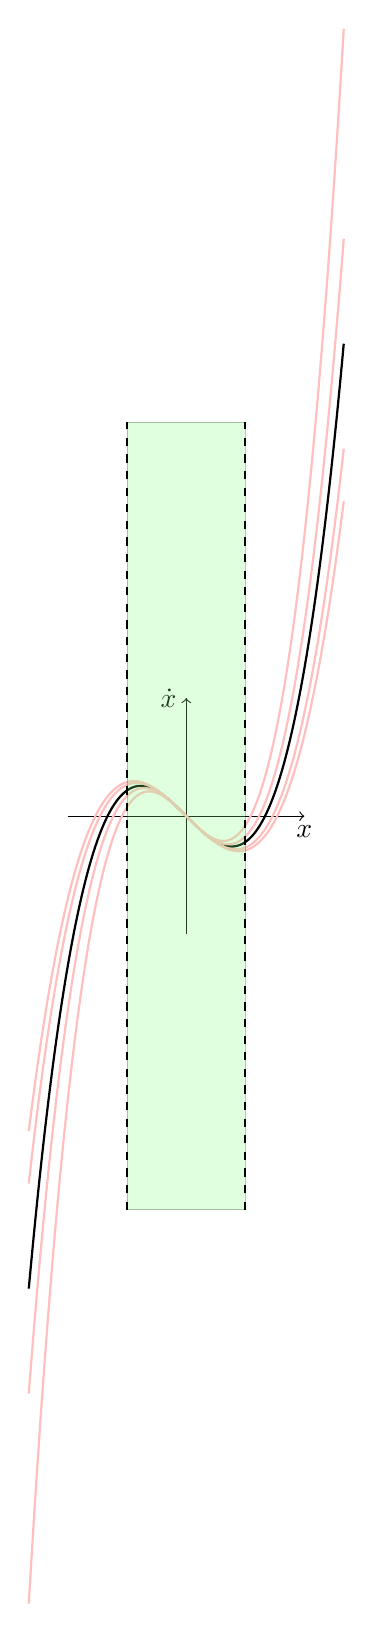
\begin{tikzpicture}[domain=-2:2,samples=400]
    \draw[->] (-1.5,0) -- (1.5,0) node[below] {$x$};
    \draw[->] (0,-1.5) -- (0,1.5) node[left] {$\dot{x}$};
    % \foreach \i in {-1,1} {
    %     \draw (\i,.1) -- (\i,-.1) node[below] {$\i$};
    % }

    % \foreach \i in {-1,1} {
    %     \draw (.1,\i) -- (-.1,\i) node[left] {$\i$};
    % }

    \draw[black, thick] plot (\x,{-\x + \x*\x*\x});

    \foreach \w in {3/4, 5/6, 7/6, 3/2} {
      \draw[pink, thick] plot(\x, {-\x + \w*\x*\x*\x});
    }

    % Fill the region of attraction
    \draw[fill=green!50, nearly transparent] (-.75,-5) -- (-.75,5) -- (.75,5) -- (.75,-5) -- cycle;

    % Draw the dashed lines around the region of attraction.
    \draw[dashed, thick, black] (-.75,-5) -- (-.75,5);
    \draw[dashed, thick, black] (.75,-5) -- (.75,5);

    % \draw[red] (-1,0) circle [radius=6pt];
    % \draw[red] (1,0) circle [radius=6pt];
    % \filldraw (0,0) circle [radius=3pt];
\end{tikzpicture}
\end{document}
  \caption[The region of attraction for the system \(\dot{x} = -x + wx^3\)]{The
    region of attraction for the system \(\dot{x} = -x + wx^3\), where \(w\) is
    a bounded uncertainty parameter.}
\end{figure}

Moving on to the most important topic for this thesis -- the analysis and
verification of regions of attraction in the presence of uncertainty. The
general idea is based around \textit{common Lyapunov functions}, which, in
contrary to regular Lyapunov analysis searches for a function which is negative
for \textit{all values of \(w\) and \(x\)}, as opposed to all values of \(x\).
\begin{example}{One-dimensional system with gain uncertainty}
  Given the same nonlinear dynamic system as in \cref{subsec:Estimating the
    region of attraction for a one-dimensional system}, but with a
  \textit{bounded uncertainty term} \(w\), with
  \[
    \dot{x} = -x + wx^3, \; w_{min} \leq w \leq w_{max}
  \]
\end{example}
here the origin is still stable, but the \textit{robust region of attraction} is
smaller than it was without uncertainty. By using the same Lyapunov candidate as
above, \(V(x) = \frac{1}{2}x^2\),
\[
  \dot{V}(x) = \frac{\partial V}{\partial x_i} f_i(x) = x(-x + wx^3) = -x^2 +
  wx^4.
\]
Which, when analyzed yields
\begin{align*}
  \dot{V}(x) &< 0 \\
  -x^2 + wx^4 &< 0 \\
  x^2 &> wx^4
\end{align*}
or equivalently
\[
  \abs{x} < \frac{1}{\sqrt{w_{max}}} = \sqrt{\frac{2}{3}}.
\]
Which shows that \(\abs{x} < \sqrt{\frac{2}{3}}\) is inside the \textit{robust
  region of attraction} for the uncertain gain system. At other times the fixed
points of the uncertain system might be unknown. Still, it is possible to employ
Lyapunov functions to give guarantees about the behavior of the system. For this
thesis this idea will be employed to stabilize a simple airplane model around a
nominal trajectory, thus it is not so important that the airplane sticks exactly
to the path, as long as there exists some convergence guarantees around it. The
extension, where one verifies the stability of a trajectory instead of a fixed
point is done through giving the Lyapunov function a time parameter, so that the
origin moves along the trajectory along with the dynamical system. Next, the
\ac{SOS} framework is applied to a \textit{Additive noise system}, which is what
\cref{eq:model-dynamics} is.

\begin{example}{Additive noise system}
  Next, consider the same system with added noise \(\dot{x} = -x + x^3 + w\),
  \(-\frac{1}{4} \leq w \leq \frac{1}{4}\). As noted previously, the fixed point
  is not at the origin for all values of \(w\), it moves depending on the value.
  However, an invariant set argument can be used to guarantee that the the
  uncertain dynamical system will stay near the origin if it starts near the
  origin.
\end{example}

\begin{figure}
  \centering
  \documentclass[tikz,border=3mm]{standalone}
\begin{document}
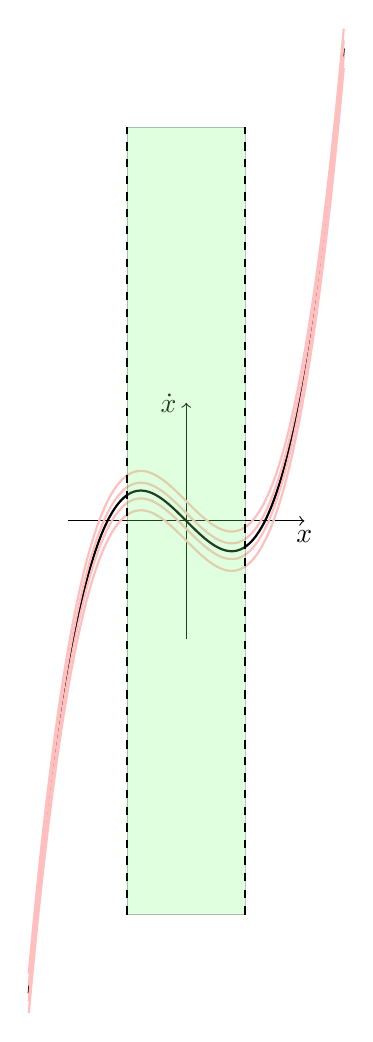
\begin{tikzpicture}[domain=-2:2,samples=400]
    \draw[->] (-1.5,0) -- (1.5,0) node[below] {$x$};
    \draw[->] (0,-1.5) -- (0,1.5) node[left] {$\dot{x}$};
    % \foreach \i in {-1,1} {
    %     \draw (\i,.1) -- (\i,-.1) node[below] {$\i$};
    % }

    % \foreach \i in {-1,1} {
    %     \draw (.1,\i) -- (-.1,\i) node[left] {$\i$};
    % }

    \draw[black, thick] plot (\x,{-\x + \x*\x*\x});

    \foreach \w in {-1/4, -1/10, 1/10, 1/4} {
      \draw[pink, thick] plot(\x, {-\x + \x*\x*\x + \w});
    }

    % Fill the region of attraction
    \draw[fill=green!50, nearly transparent] (-.75,-5) -- (-.75,5) -- (.75,5) -- (.75,-5) -- cycle;

    % Draw the dashed lines around the region of attraction.
    \draw[dashed, thick, black] (-.75,-5) -- (-.75,5);
    \draw[dashed, thick, black] (.75,-5) -- (.75,5);

    % \draw[red] (-1,0) circle [radius=6pt];
    % \draw[red] (1,0) circle [radius=6pt];
    % \filldraw (0,0) circle [radius=3pt];
\end{tikzpicture}
\end{document}
  \caption[The region of attraction for the system \(\dot{x} = -x + x^3 + w\)]{The region of attraction for the system \(\dot{x} = -x + x^3 + w\),
    where \(w\) is a bounded uncertainty parameter.}
\end{figure}

Once again, applying the same Lyapunov function \(V(x) = \frac{1}{2}x^2\),
\[
  \dot{V}(x) = \frac{\partial V}{\partial x_i} f_i(x) = x(-x + x^3 + w) = -x^2 +
  x^3 + wx.
\]
However, the invariant set argument here is a little different, as every
sub-level set of the Lyapunov function is not invariant. For instance \(V \leq
\frac{1}{3}\) is a \textit{robust invariant set}, because if \(V =
\frac{1}{3}\),
\[
  \forall w \in \left[ w_{min}, w_{max} \right], \; \dot{V}(x,w) < 0.
\]
Thus, \(V(x)\) can never start out at less than \(\frac{1}{3}\), and obtain
values greater than \(\frac{1}{3}\).
\[
  V = \frac{1}{3} \implies x = \pm \sqrt{\frac{2}{3}} \implies \dot{V} =
  -\frac{2}{9} \pm w \sqrt{\frac{2}{3}} < 0, \; \forall w \in \left[
    -\frac{1}{4}, \frac{1}{4} \right].
\]
However, note that \(V = \frac{1}{32}\) yields
\[
  V = \frac{1}{32} \implies x = \pm \frac{1}{4} \implies \dot{V} = -\frac{1}{4}
  + \frac{1}{16} \pm w\frac{1}{4}, \; \not \forall w \in \left[ -\frac{1}{4},
    \frac{1}{4} \right].
\]
Which shows that not all sub-level sets of an invariant set is invariant in the
case of additive uncertainty, so the conclusion is that it is not robustly
invariant. Through the \ac{SOS} procedure and the Lyapunov function theory
outlined, a \ac{SOS} program for verifying the dynamical system utilized in the
examples looks like

\begin{example}{Region of attraction for the one-dimensional cubic system}
  \[
    \dot{x} = -x + x^3
  \]
  Using the Lyapunov function candidate \(V = x^2\), and the multiplier
  polynomial \(L(x) = \alpha_0 + \alpha_1x + \alpha_2x^2 + \alpha_3x^3 +
  \alpha_4x^4\), the \ac{SOS} optimization problem can be defined as
  \begin{align*}
    \text{find } \alpha& \\
    \text{subject to }& -\dot{V}(x) - L(x)\left( 1 - V(x) \right) \; &\text{is SOS} \\
                       & &L(x) \text{ is SOS}.
  \end{align*}
  Which written in \textit{YALMIP}~\cite{Lofberg2004,Lofberg2009} yields the
  \ac{SOS} program in \cref{fig:sos-program-additive}.
\end{example}

\begin{figure}
  \centering
  \lstinputlisting[language=matlab]{figures/preliminaries/cubicregionofattraction.m}
  \label{fig:sos-program-additive}
\end{figure}

\subsubsection{Robust Set-Invariance}

A sub-level set of the Lyapunov function is, in comparison with the system
without uncertainties, not guaranteed that every sub-level set of the Lyapunov
function is not necessarily invariant. (Give example.).

